\onehalfspacing

\chapter{Conclusion and outlook}

\label{chap:Chapter_6}

In this thesis, we developed a fast and efficient numerical model to simulate dynamics of phase separated droplets in large-scale emulsions in the presence of chemical reactions and chemical gradients, circumventing the need of solving the computationally expensive \textit{Cahn-Hilliard} equation; see Refs. \cite{Review2019,CahnHilliardEq,Cahn1958}, describing phase separation.
We were motivated from numerous examples from biology, specifically biological cells, which need to organize their intracellular environment in a precisely regulated spatiotemporal manner to properly function and survive.
One way the cell achieves this is through manufacturing membrane-less organelles (or condensates) in an energetically efficient way using Liquid-liquid phase separation.
Additionally, aberrant condensates; which form via poor spatiotemporal regulation by the cell, are implicated in many diseases, a few being: familial amyotrophic lateral sclerosis (fALS), frontotemporal lobar degeneration (FTLD); see Ref. \cite{QAMAR2018720}, amyotrophic lateral sclerosis (ALS); see Ref. \cite{Mateju2017} and Alzheimer’s disease; see Refs. \cite{Williams2006,Mucke2009}.
This precise control of the cell over it's condensates is thought to be accomplished through various mechanisms, a few being: utilizing chemical gradients, chemical reactions via PTMs, regulating pH and temperature, physically modifying it's internal environment through forming networks and using pickering agents to modify the surface properties of the condensates.

We were interested disentangling and separately investigating the roles of two important mechanisms out of the above, namely chemical reactions and external chemical gradients, through numerical simulations of dynamics of phase separated droplets.
However, simulating the traditional \textit{Cahn-Hilliard} equation of phase separation (continuous model given by \Eqref{eqn:CHActive}) for large systems in three dimensions is prohibitively costly, as small time steps and fine grid discretizations have to be used.
Earlier works have improved the computational speeds of this model using approaches such as using multi-grid methods; see Ref. \cite{Lee2021_CH_model}, finite element modelling; see Refs. \cite{zhou2015, Chen2021}, incorporating meshless methods; see Ref. \cite{MOHAMMADI2019919} and adaptive grids; see Refs. \cite{BANAS20082,Ceniceros2007}, to overcome the challenges posed, but the fundamental drawbacks still persist.

However, since we are interested primarily in modelling dynamics of droplets, we circumvented these problems by focusing only on phase separation inside the nucleation and growth regime, and assuming that sufficiently finite perturbations have already nucleated droplets.
We discussed the thin-interface approximation; see \Eqsref{eqn:thin_interface_model}, which was a coarse-grained analytical formulation of the continuous model subject to strong phase separation, low variation of volume fractions in the droplet phase and the dilute phase themselves and large droplet sizes compared to the interface width.
This approximation describes dynamics of droplets and dynamics of the dilute phase separately, instead of the full volume fraction field from the continuous model; see \figref{fig:schematics}, thus effectively `de-coupling' the description of phase separated droplets from the dilute phase.
This analytical approach was utilized by Zwicker et al. \cite{Zwicker2015} to study kinetics of many droplet systems and effects of chemical reactions on such systems.

The aim of this thesis was to then utilize the thin-interface approximation, build a numerical model (the effective droplet model) upon it to simulate the dynamics of phase separated droplets in presence of chemical reactions and external chemical gradients, and thus obtain insights how the cell is able to robustly regulate the size and shape of the condensates in spite it's complex intracellular environment which experiences thousands of biomolecular reactions every second.
Using the thin-interface approximation, we built up the effective droplet model systematically and chose optimum values for various simulation parameters based on comparisons with simulations using the continuous model.
We then demonstrated that the effective droplet model captures droplet dynamics accurately for two extreme scales, namely a) simple scenarios typically involving a single droplet or a pair of droplets and b) \textit{Ostwald-Ripening} of $10^5$ droplets, where it accurately replicates the theoretical predictions for the $t^{1/3}$ scaling of the mean radius from Refs. \cite{LSWanalytics,Lifshitz}.
In addition, we studied the roles of two important mechanisms that influence the physics of phase separation - chemical reactions and external chemical gradients on droplet dynamics, by simulating them individually and thus disentangling their effects on growth and drift of droplets.

We now reasonably assume that with optimum choices for the simulation parameters; as described in Chapter \ref{chap:Chapter_4}, intermediate-scale scenarios (which are computationally expensive to be simulated using the continuous model), for example, many-droplet systems in the presence of chemical reactions and chemical gradients, should also be captured well using the effective droplet model, which we will demonstrate and discuss next.

\section{Droplet dynamics in the presence of chemical reactions and external volume fraction gradient}

We now present the final demonstration of the effective droplet model, where we simulate the combined effect of chemical reactions and external volume fraction gradients on the dynamics of the droplets; see \figref{fig:active_emulsion_gradient}.
We simulate many active droplets in a large three dimensional system and the droplets are immersed in an external volume fraction gradient (along one dimension) of the droplet material.
Based on results from Chapter \ref{chap:Chapter_5}, we expect the droplets to drift in the direction of the gradient.
Additionally, as seen from Chapter \ref{chap:Chapter_5}, droplets with first-order reactions (and in the absence of an external gradient) attain a stable radius $\overline{R}_\mathrm{3D}$ in three dimensions, which is based on flux balances and given by numerically solving for $\jIn = \jOut$ from \Eqref{eqn:fluxes_in_firstorder}.
Hence, we hypothesize the following: if we want to achieve \textit{both}: stable radii (size control) and droplet drift (position control) for the droplets, chemical reactions and external chemical gradients might be the right combination to materialize such a situation. 

To investigate our claim, we now simulate four droplets with radii chosen uniformly in $[0.8 \left \langle R_0 \right \rangle, 1.2 \left \langle R_0 \right \rangle]$, where $\left \langle R_0 \right \rangle = 40w$.
The droplets are placed in cubic domain of size $[0, L]^3$ with $L = 10^3 w$ with $\dx \approx \ell \approx \Delta s \approx \left \langle R_0 \right \rangle$; see \figref{fig:active_emulsion_gradient}, along with the boundary conditions $\phiOut(x = -L/2) = 0$ and $\phiOut(x = L/2) = 0.1$ to maintain the one-dimensional gradient and no-flux boundary conditions at the remaining system boundaries.
\begin{figure}[tb]
\centering
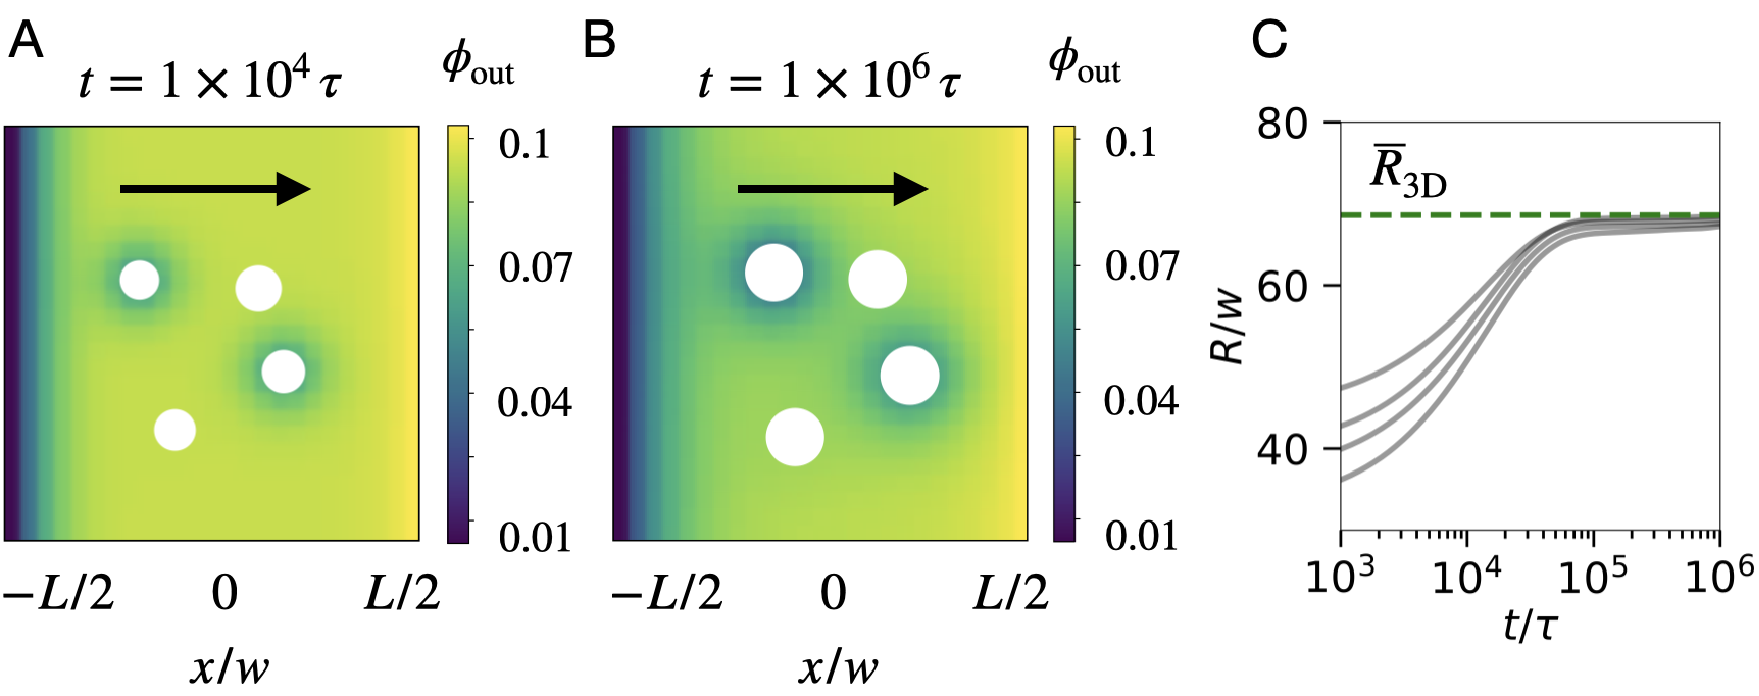
\includegraphics[scale=0.52]{MainContent/Figures/active_emulsion_gradient.pdf}
\vspace{10pt}
\caption{\textbf{Active droplets ripening along external gradients in three dimensional systems.}
Figure shows ripening of active droplets in three dimensional systems at intermediate snapshots, using effective droplet model. Droplets (white circles) are shown as two dimensional projections and arrow shows the direction of the gradient along which the droplets grow and drift.
\mbox{(A-B)} Active droplets with first-order chemical reactions under the influence of an external volume fraction (one-dimensional) gradient grow towards a fixed size and drift towards the gradient direction, thus qualitatively depicting spatiotemporal size control of biomolecular condensates.
The gradient is maintained only along the $x$ direction through boundary conditions.
(C) Droplet radius $R$ as a function of time $t$ for different droplets approaching a fixed size $\overline{R}_\mathrm{3D}$ (dashed line), which is obtained from numerically solving for $\jIn = \jOut$ from \Eqsref{eqn:fluxes_in_firstorder}; ; compare to \figref{fig:active_emulsions}.
4 droplets with radii chosen uniformly in $[0.8 \left \langle R_0 \right \rangle, 1.2 \left \langle R_0 \right \rangle]$, where $\left \langle R_0 \right \rangle \approx 40 w$ are placed in cubic Cartesian domain of size $[0, L]^3$ with $L = 10^3 w$ with $\dx \approx \ell \approx \Delta s \approx \left \langle R_0 \right \rangle$ along with the boundary conditions $\phiOut(x = -L/2) = 0$ and $\phiOut(x = L/2) = 0.1$ and no-flux boundary conditions at the remaining system boundaries.
Model parameters are $s(\phi)= \kf (1 - \phi) - \kb \phi$, $\phiOut(t=0) =\phi_\infty$, $\kf = 1 \times 10^{-5} \tau^{-1}$ and $\kb = 1 \times 10^{-4} \tau^{-1}$.
Remaining parameters are specified in Fig. \ref{fig:droplet_pair_schematics}.
}
\label{fig:active_emulsion_gradient}
\end{figure}
Indeed as seen from \figref{fig:active_emulsion_gradient}, we observe that droplets (shown as two dimensional projections) grow as they drift along the (one dimensional) gradient \textit{and} they approach the fixed radius given by $\overline{R}_\mathrm{3D}$, thus achieving both - size control and droplet drift.
Thus, through simulations of the effective droplet model, we are able to qualitatively demonstrate spatiotemporal size control of biomolecular condensates, where precise location and size is controlled by the cell potentially through chemical gradients and chemical reactions; see Refs. \cite{Brangwynne2009,Brangwynne2013}.

\section{Future extensions to the effective droplet model}

Having modelled the effects of chemical reactions and external chemical gradients on droplet dynamics, we now discuss and propose future improvements for the effective droplet model.
This model has been extended to integrate elasticity and utilized by Vidal-Henriquez et al. \cite{VidalHenriquez2021,Vidal2020} to study droplet ripening in passive emulsions with the presence of an elastic matrix.
This is a valuable extension to the model, as cells are thought to utilize chromatin networks to suppress coalescence of condensates and thus stabilizing them; see Refs. \cite{Feric2013,Wiegand2020,Boeddeker2022}.
Additional extensions such as fluid flows which are pertinent to biological cells; see Refs. \cite{Brangwynne2009,Setru2021,Brangwynne2011}.
In particular, Seyboldt et al. \cite{Seyboldt_2018} investigated the role of hydrodynamic flows in stabilizing droplets in presence of strong chemical reactions.
Fluid flows can be incorporated by including advection terms in the dynamics of volume fractions inside the droplets and in the background field.

Further, we currently have ignored the effects of droplet splitting and coalescence.
Coalescence can be incorporated in the model through volume conservation of droplets touching each other.
Inside biological cells, condensates have been shown to exhibit anomalous coarsening behaviour, primarily due to hindrance and physical barrier which curb their ability of coalesce; see Refs. \cite{Feric2013,Quiroz2020,Boeddeker2022,Lee2021}.
Thus including the effects of droplet coalescence in the model will be a useful extension.
Droplet splitting along with non-spherical droplets will also be a valuable addition to the model, as it is relevant when considering strong chemical reactions; see Refs. \cite{Zwicker_nature_2016,Seyboldt_2018}.

Taken together, we demonstrated that the effective droplet model faithfully captures the effects of chemical reactions and external chemical gradients on droplet dynamics.
Additionally, the gain in computational speed of the effective droplet model is shown to be orders of magnitude faster than simulations of the continuous model given by \Eqref{eqn:CHActive} for similar systems, making it a viable and a pragmatic option for fast and computationally efficient simulations of phase separated droplets in large many-droplet emulsions.
Most importantly, our model can be used as a modular platform, which can be extended to include other relevant physical phenomena which play a role in controlling condensate dynamics, thus shedding insights on the formation, dissolution, stability and sizes of biomolecular condensates.
